We begin by providing an overview of canonical correlation analysis (CCA). For
completeness and ease of future derivations, we derive the solution for CCA from first
principles. We then give an overview of previous work on CCA in the sample starved regime,
summarizing the results of \cite{pezeshki2004empirical,nadakuditi2011fundamental}. We
conclude by providing new results based on the observations in
\cite{nadakuditi2011fundamental}.

\section{Mathematical Formulation of CCA}\label{sec:cca_form}
Assume that observations $\yI\in\complex^{d_1}$, $\yII\in\complex^{d_2}$
are drawn from two distributions $\yI\sim\mathcal{Y}_1$,
$\yII\sim\mathcal{Y}_2$. Furthermore, assume that the distributions have zero mean,
\textit{i.e.} $\E{\yI}=\E{\yII}=0$. We will use the following notation for the covariance
matrices of the distributions: $\E{\yI\yI^H}=\RI$, $\E{\yII\yII^H}=\RII$,
$\E{\yI\yII^H}=\RIII$.

The goal of CCA is to find a linear transformation for each dataset that maximizes the
correlation between the datasets in the projected spaces. We represent the linear
transformations with the canonical vectors $\xI\in\complex^{d_1}$ and
$\xII\in\complex^{d_2}$ and the projection with the canonical variates $\wI=\xI^H\yI$ and
$\wII=\xII^H\yII$. The objective is to find the canonical vectors $\xI$ and $\xII$ that
maximize the correlation between the canonical variates $\wI$ and $\wII$. Formally, the
optimization problem is
\begin{equation}\label{eq:cca_opt}
  \begin{aligned}
    &\argmax_{\xI,\xII}&&\rho = \E{\wI\wII}\\
    & \text{subject to}&&\E{\wI^2}=1, \E{\wII^2}=1.
  \end{aligned}
\end{equation}
Substituting the expressions for the canonical variates and the correlation matrices, this
optimization problem may be written as
\begin{equation}\label{eq:cca_opt2}
  \begin{aligned}
    &\argmax_{\xI,\xII}&&\rho = \xI^H\RIII\xII\\
    & \text{subject to}&&\xI^H\RI\xI=1, \xII^H\RII\xII=1.
  \end{aligned}
\end{equation}

The Lagrangian used to solve (\ref{eq:cca_opt2}) is
\begin{equation}\label{eq:cca_lagr}
  L(\xI,\xII,\lambda_1,\lambda_2) = \xI^H\RIII\xII - \lambda_1(\xI^H\RI\xI -1) - \lambda_2(\xII^H\RII\xII-1).
\end{equation}
Solving (\ref{eq:cca_opt2}) is achieved by setting the partial derivatives of
(\ref{eq:cca_lagr}) equal to zero. Doing so yields 
\beq\label{eq:cca_partials}\ba
& 0 && = \RIII\xII -2\lambda_1\RI\xI\\
& 0 && = \RIII^H\xI -2\lambda_2\RII\xII.\\
\ea\eeq 
By left multiplying the first equation of (\ref{eq:cca_partials})by $\xI^H$ and
the second equation by $\xII^H$ and using the definitions and constraints in
(\ref{eq:cca_opt2}), 
\beq\label{eq:cca_rho} 
\rho = 2\lambda_1=2\lambda_2.
\eeq 
Therefore, the Lagrange multipliers are equal and the value of the maximum correlation
between the datasets is a multiple of the Lagrange multiplier. Solving one equation in
(\ref{eq:cca_partials}) for $\xII$ and substituting in the other results in the following
eigenvalue system
\cite{nielsen2002multiset,nadakuditi2011fundamental,welling2005kcca,kettenring1971canonical,nielsen1994analysis}
\begin{equation}\label{eq:cca_eigval_sys}
  \RI^{-1}\RIII\RII^{-1}\RIII^H\,\xI = \rho^2\xI
\end{equation}
with the relationship
\beq\label{eq:x2}
\xII=\frac{1}{\rho}\RII^{-1}\RIII^H\,\xI.
\eeq

Solving (\ref{eq:cca_eigval_sys}) for the eigenvector corresponding to the largest
eigenvalue solves (\ref{eq:cca_opt2}). Substituting this eigenvalue/eigenvector pair in
(\ref{eq:x2}) gives the complete solution $\left(\xI,\xII,\rho\right)$ for the transformations
  and maximum correlation between the datasets. Multiple canonical basis vectors may be
  found by recursively finding the next largest eigenvalue and corresponding eigenvector
  in (\ref{eq:cca_eigval_sys}). In many learning applications, it is common to project
  onto multiple canonical basis vectors.

 Using a similarity transform, we can frame the eigen-system in (\ref{eq:cca_eigval_sys})
 as an SVD problem. Define $f = \RI^{1/2}\xI$ and $g=\RII^{1/2}\xII$. Then
 (\ref{eq:cca_eigval_sys}) may be rewritten as
\begin{equation}\label{eq:eigval_sys2}
  \RI^{-1/2}\RIII\RII^{-1}\RIII^H\RI^{-H/2}f = \rho^2f.
\end{equation}
Defining $C=\RI^{-1/2}\RIII\RII^{-H/2}$, (\ref{eq:eigval_sys2}) can be rewritten as
\begin{equation}\label{eq:cca_C_eigval}
  CC^Hf=\rho^2f.
\end{equation}

Clearly, from (\ref{eq:cca_C_eigval}), we may obtain a closed form solution for $f$ and
$\rho$ through the SVD of $C$. Let $FKG^H$ be the SVD of $C$ where
$F=[f_1,\dots,f_{d_1}]$, $K\in\complex^{d_1\times
  d_2}=\diag(k_1,\dots,k_{\min\left(d_1,d_2\right)})$, and $G=[g_1,\dots,g_{d_2}]$. Then the solution
for the canonical vector pair corresponding to the largest canonical correlation is
\beq\label{eq:cca_svd_sol}\ba
&\rho = k_1\\
&\xI = \RI^{-1/2}f_1\\
&\xII = \RII^{-1/2}g_1.\\
\ea\eeq

\section{Empirical CCA}\label{sec:emp_cca}

The above analysis assumes that the covariance matrices $\RI$, $\RII$, and $\RIII$ are all
known. However, in most applications these covariance matrices are unknown and must be
estimated from data. In such an empirical setting, we assume that we are given $n$
observations, or samples, from each dataset $\yI^{(i)}$ and $\yII^{(i)}$ for
$i=1,\dots,n$. We may stack these observations in training data matrices
\be
Y_1=\left[\yI^{(1)},\dots,\yI^{(n)}\right], \text{ and } 
Y_2=\left[\yII^{(1)},\dots,\yII^{(n)}\right].
\ee
Using these training data matrices, the sample covariance matrices are
\beq\label{eq:scm}\ba
&\RIhat = \frac{1}{n} Y_1Y_1^H\\
&\RIIhat = \frac{1}{n} Y_2Y_2^H\\
&\RIIIhat = \frac{1}{n} Y_1Y_2^H.\\
\ea\eeq
We may then substitute these covariance matrix estimates in the expression for $C$,
resulting in the estimator
\beq\label{eq:cca_Chat}
\widehat{C} = \RIhat^{-1/2}\RIIIhat\RIIhat^{-1/2}.
\eeq
Defining $\widehat{C} =\widehat{F}\widehat{K}\widehat{G}^H$ as the SVD of $\widehat{C}$,
the solution to empirical CCA is
\beq\label{eq:cca_svd_sol}\ba
&\widehat{\rho} = \widehat{k}_1\\
&\xIhat = \RIhat^{-1/2}\,\widehat{f}_1\\
&\xIIhat = \RIIhat^{-1/2}\,\widehat{g}_1.\\
\ea\eeq

\section{Performance of Empirical CCA}

Here, we present the relevant works that explore the performance of empirical CCA and
demonstrate how they provide insight to the data fusion questions posed herein. First, we
note that to construct $\widehat{C}$ in (\ref{eq:cca_Chat}) we must invert $\RIhat$ and
$\RIIhat$. However, if the number of samples $n$ is less than either of the data
dimensions $d_1$ or $d_2$, then the sample covariances are not invertible. In this case, a
regularized version of CCA is often employed. We discuss this in depth in Chapter
\ref{sec:rcca}.

\subsection{Performance Breakdown When $n<d_1+d_2$}
Pezeshki et al. analyze the performance of empirical CCA in the sample poor regime when
$n<d_1+d_2$ in \cite{pezeshki2004empirical}. In particular, they show that in this regime,
empirical CCA breaks down completely; the leading singular value of $\widehat{C}$ is 
deterministically 1. Below we provide a different proof of this result.

Let $Y_1 = U_1\Sigma_1 V_1^H$ and $Y_2=U_2\Sigma_2V_2^H$ be the data SVDs of our training
data matrix. Using this notation, 
\beq\label{eq:cca_chat_svd}\ba
& \widehat{C} &&= \RIhat^{-1/2}\RIIIhat\RIIhat^{-1/2}\\
&&&  = \left(Y_1Y_1^H\right)^{-1/2}Y_1Y_2^H\left(Y_2Y_2^H\right)^{-1/2} \\
&&& = \left(U_1\Sigma_1\Sigma_1^HU_1^H\right)^{-1/2}U_1
\Sigma_1V_1^HV_2\Sigma_2^HU_2^H\left(U_2\Sigma\Sigma_2\Sigma_2^H\right)^{-1/2}\\
&&& = U_1 I_{d_1\times n}V_1^HV_2I_{n\times d_2}U_2^H\\
\ea\eeq
Therefore, we can conclude that since $U_1$ and $U_2$ are unitary matrices,
\be \widehat{\rho} = \widehat{k}_1 = \sigma_1\left(\widehat{C}\right) =
\sigma_1\left(\bar{V}_1^H \bar{V}_2\right) 
\ee
where $\bar{V}_1=V(:,1:\min\left(d_1,n\right))$, $\bar{V}_2 =
V(:,1:\min\left(d_2,n\right))$, and $\sigma(\cdot)$ returns the largest singular value of
the provided matrix. These (possibly) trimmed matrices have orthonormal columns and thus
form a basis for a subspace. Consider the case when $n<d_1+d_2$. If $n<d_1$ or $n<d_2$,
then either $\bar{V}_1$ or $\bar{V}_2$ is a unitary matrix and so
$\sigma_1\left(\bar{V}_1^H\bar{V}_2\right)=1$ deterministically. In the case when
$\max\left(d_1,d_2\right)<n<d_1+d_2$, $\bar{V}_1$ is a dim-$d_1$ subspace of $\complex^n$ and
$\bar{V}_2$ is a dim-$d_2$ subspace of $\complex^n$. However, because $n<d_1+d_2$, these
subspaces are \textit{guaranteed} to intersect. Let $v$ be the shared basis vector of the
subspaces defined by $\bar{V}_1$ and $\bar{V}_2$. Therefore, we can express these
subspaces using the bases $\bar{V}_1=\left[v\,\, v^{\perp}_{\bar{V}_1}\right]$ and
$\bar{V}_2 = \left[v\,\,  v^{\perp}_{\bar{V}_2}\right]$. Therefore
\be
\bar{V}_1^H\bar{V}_2 = \left[\begin{array}{c}v^H
    \\v^{H\perp}_{\bar{V}_1}\end{array}\right]\left[v \,\,
  v^{\perp}_{\bar{V}_2}\right] = \left[\begin{array}{cc}1 & 0^H \\ 0 &
    v^{H\perp}_{\bar{V}_1}v^{\perp}_{\bar{V}_2}\end{array}\right]. 
\ee
This matrix clearly has a largest singular value of 1.

Therefore, when $n<d_1+d_2$,
$\widehat{\rho}=\widehat{k}_1=\sigma_1\left(\widehat{C}\right)=1$ deterministically. This
is an extremely undesirable property of empirical CCA. When $\widehat{\rho}=1$, it implies
that the canonical vectors provide a transformations that result is perfect (colinear)
correlated canonical variates. This property holds for all distributions and any possible
data matrices $Y_1$ and $Y_2$ even if the datasets contain no correlated signals.

\subsection{Simulation Results}

We now demonstrate this phenomena through a series of simulations. While some of these
results reproduce previous work, they are needed to form a basis for comparison to
new algorithms. In this setup, we consider two cases. In the first, both datasets are
simply Gaussian noise. In the second, each dataset contains a noisy low-rank signal that is
correlated with the other dataset. The data model for this setup is

\beq\label{eq:cca_data_model1}\ba
\text{Noise:}\begin{cases}
\yI^{(i)}=\mathcal{N}\left(0,I_{d_1}\right) & \\
\yII^{(i)}=\mathcal{N}\left(0,I_{d_2}\right) & \\
\end{cases}
\text{Signal:}\begin{cases}
\yI^{(i)}=\sigma u_1 z_1^{(i)} + \mathcal{N}\left(0,I_{d_1}\right) & \\
\yII^{(i)}=\sigma u_2 z_2^{(i)} + \mathcal{N}\left(0,I_{d_2}\right) & \\
\end{cases}
\ea\eeq
where $u_1\in\complex^{d_1}$ and $u_2\in\complex^{d_2}$ are unit norm signal
vectors, $\sigma>0$ is a SNR, and 
\be 
z^{(i)}=\left[\begin{array}{c}z_1^{(i)} \\  z_2^{(i)}\end{array}\right]\sim
\mathcal{N}\left(0,\left[\begin{array}{cc} 1 & \rho \\ \rho & 1\end{array}\right]\right).
\ee 
All additive Gaussian noise terms are independent. We note that in this setup the SNR,
$\sigma$, is the same for both datasets. This would usually not be the case and we could
run these simulations using a $\sigma$ unique to each dataset, however, we wish to reduce
the number of parameters in the simulation.

For $i=1,\dots,n$ we produce $n$ samples for each dataset under both the signal and noise
model in (\ref{eq:cca_data_model1}), resulting in four datasets $Y_1^{\text{noise}}$,
$Y_2^{\text{noise}}$, $Y_1^{\text{signal}}$, and $Y_2^{\text{signal}}$. Using the data
SVDs of $Y_1^{\text{noise}}$ and $Y_2^{\text{noise}}$ we form $\widehat{C}^{\text{noise}}$
as defined in (\ref{eq:cca_chat_svd}) and $Y_1^{\text{signal}}$ and $Y_2^{\text{signal}}$
to similarly form $\widehat{C}^{\text{signal}}$. We then take the leading singular value
of $\widehat{C}^{\text{noise}}$ and $\widehat{C}^{\text{signal}}$, resulting in two top
singular values, $\widehat{\rho}^{\text{noise}}$ and $\widehat{\rho}^{\text{signal}}$,
representing the maximum correlation in the noise datasets and the maximum correlation in
the signal datasets. This is repeated for multiple trials, where each trial generates new
datasets using different signal vectors $u_1$ and $u_2$, new $z$, and new additive
noise. This gives an empirical distribution of $\widehat{\rho}^{\text{noise}}$ and
$\widehat{\rho}^{\text{signal}}$ formed from noisy datasets and signal bearing
datasets. Figure \ref{fig:cca_errorbars} plots these empirical distributions, sweeping
over the number of training samples in each dataset for two values of $\sigma$.

\begin{figure}[h!]
  \centering
  \subfigure[$\sigma=0$ dB]{
    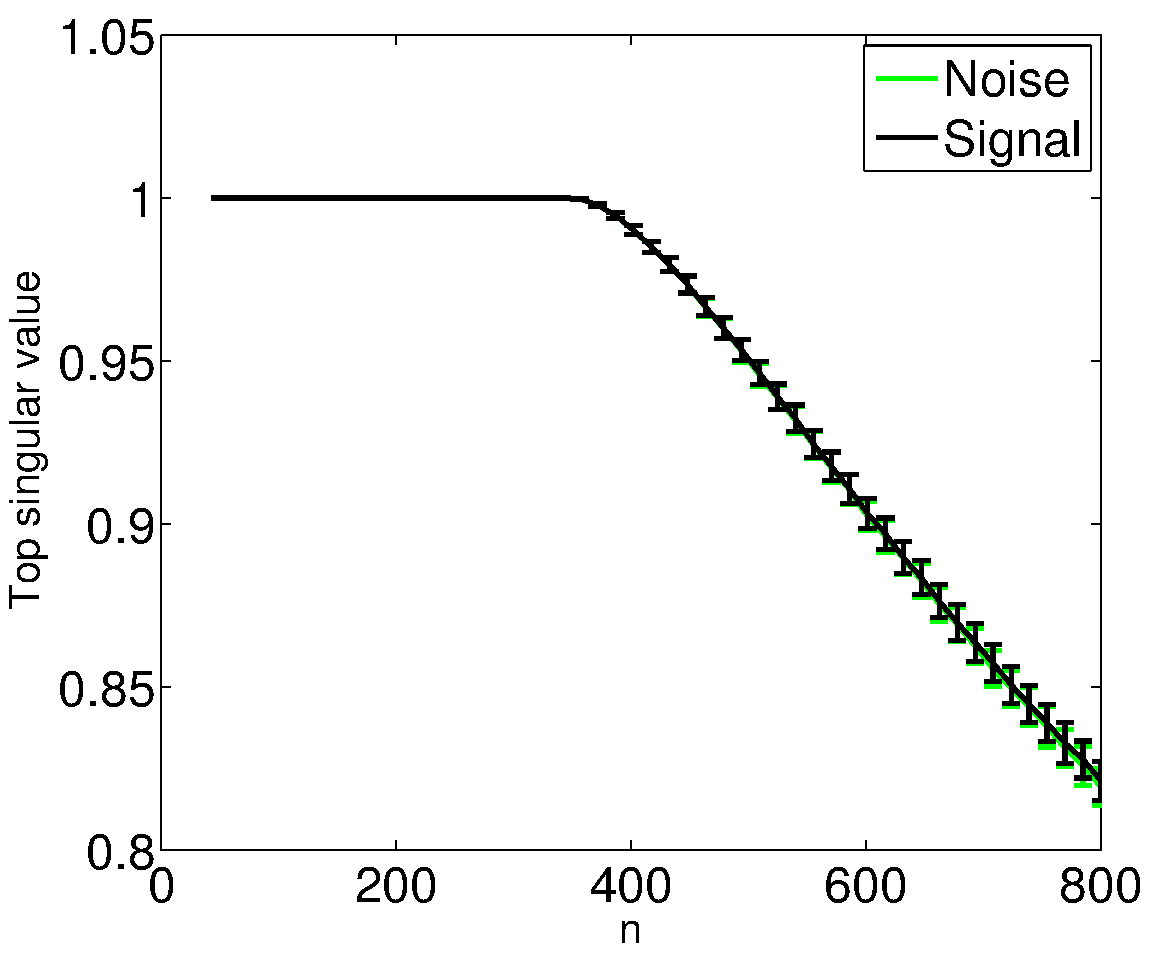
\includegraphics[width=\figwidth]{figures/cca_errorbars_low.pdf}
    \label{fig:cca_errorbars_low_snr}
  }
  \subfigure[$\sigma=3$ dB]{
    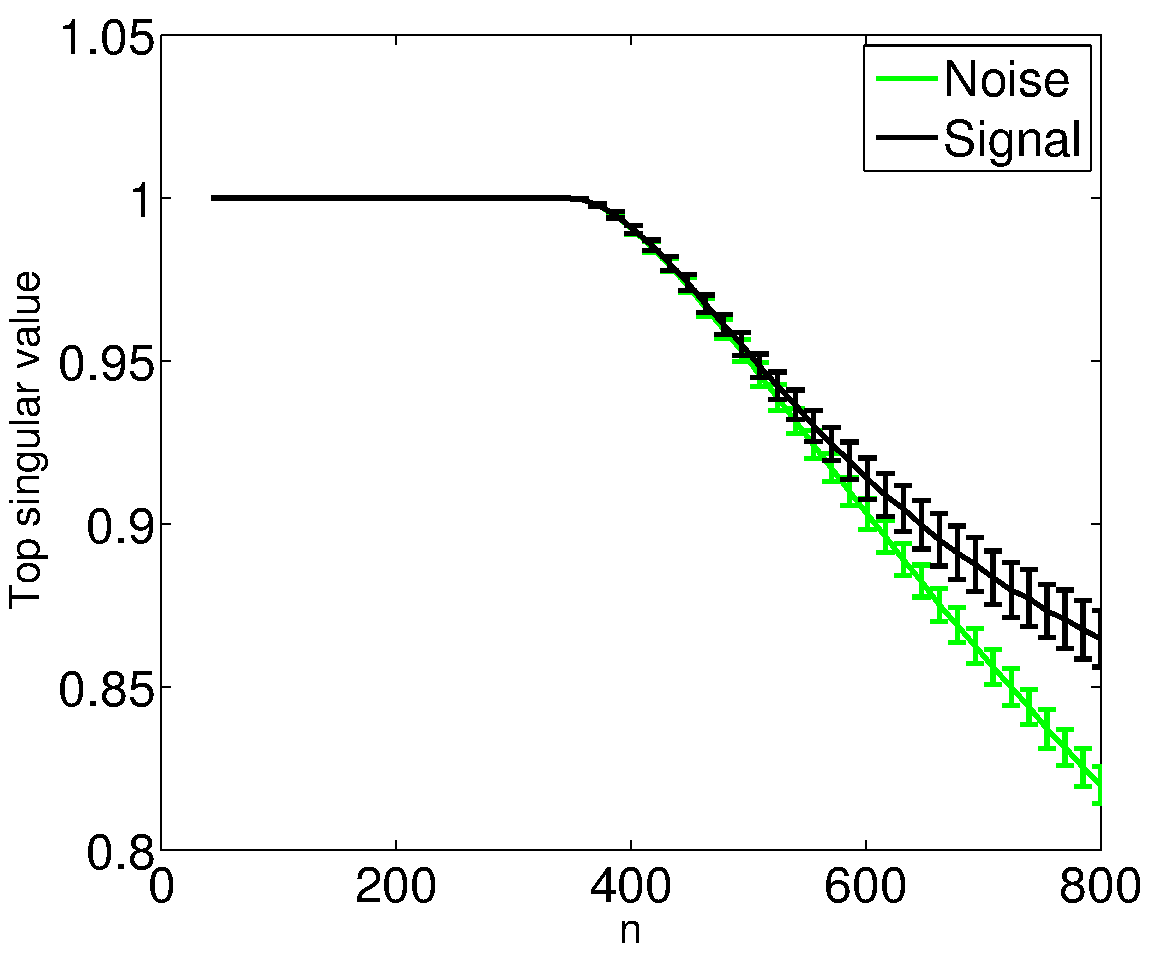
\includegraphics[width=\figwidth]{figures/cca_errorbars_high.pdf}
    \label{fig:cca_errorbars_high_snr}
  }
  \caption{Empirical distribution of the top singular value of $\widehat{C}$ in
    (\ref{eq:cca_chat_svd}) for both noise and signal data models in
    (\ref{eq:cca_data_model1}). Simulations were conducted using $d_1=200$, $d_2=150$, and
    $\rho=0.9$. The top singular value was computed for 500 trials. The mean top singular
    value is plotted with $\pm$ one standard deviation errorbars. }
  \label{fig:cca_errorbars}
\end{figure}

Figure \ref{fig:cca_errorbars} highlights the phenomena presented in
\cite{pezeshki2004empirical}. For $n<350=d_1+d_2$, $\widehat{\rho}$ is identically 1 for
both the noise and signal datasets and for both values of $\sigma$. In Figure
\ref{fig:cca_errorbars_low_snr}, the value of $\sigma$ is small enough so that even when
there are many samples present, the empirical distribution of
$\widehat{\rho}^{\text{noise}}$ follows that of $\widehat{\rho}^{\text{signal}}$. However,
when $\sigma$ is larger, as in Figure \ref{fig:cca_errorbars_high_snr}, the distributions
separate when given enough samples. A natural question to ask is ``Are these distributions
different?'' If the answer is no, then the correlation estimate returned by CCA is
useless, being unable to discern if the correlated datasets contain signal or are simply
noise. Next we reproduce the results of \cite{nadakuditi2011fundamental}, using the
two-sided Kolmorgorov-Smirnov (KS) to determine if the distributions are indeed
different. Figure \ref{fig:cca_ks_heatmap} plots the KS statistic for multiple values of
$\sigma$ and $n$.

\begin{figure}
  \centering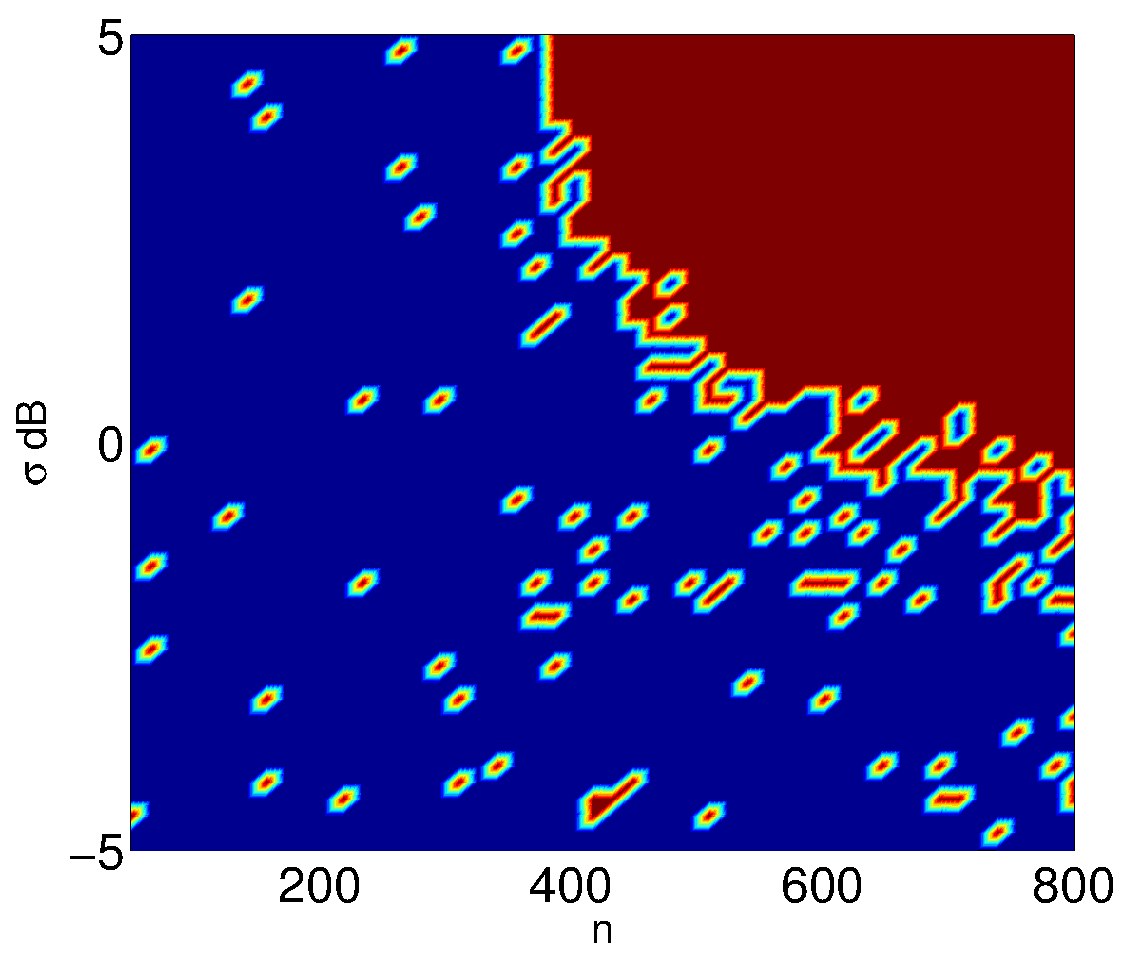
\includegraphics[width=\figwidth]{figures/cca_ks_heatmap.pdf}
  \caption{Two-sided KS statistic between the empirical distributions of the leading
    singular value of $\widehat{C}$ in (\ref{eq:cca_chat_svd}) formed from training data
    generated from the noise and signal data models in (\ref{eq:cca_data_model1}).
    Simulations were conducted using $d_1=200$, $d_2=150$, $\rho=0.9$, 500 trials, and a
    significance level of $\alpha=0.95$ for the KS test. A value of 1 indicates the
    distributions are statistically different while a value of 0 indicates the
    distributions are statistically identical.}
  \label{fig:cca_ks_heatmap}
\end{figure}

This result confirms the result in \cite{nadakuditi2011fundamental}. Two important
consequences follow from Figure \ref{fig:cca_ks_heatmap}. First, it confirms that when
$n<d_1+d_2$ CCA fails to provide meaningful correlation estimates. No matter how large the
value of $\sigma$, CCA will always return a correlation estimate of 1 for any dataset it
is provided. In this sample starved regime, CCA cannot reliably detect the presence of a
signal given two correlated datasets. Second, given $n>d_1+d_2$ samples, there is a
threshold dependent on $n$ such that when $\sigma$ is large enough, the noise and signal
distributions are statistically different and when $\sigma$ is too small, the noise and
signal distributions are statistically identical. The KS statistic determines if the
distributions are statistically distinguishable but gives no insight into \textit{how}
indistinguishable the distributions are. To explore this, we consider constructing a
na\"{\i}ve detector based on the top singular value of $\widehat{C}$. We may construct an
empirical ROC curve of such a detector using the empirical distributions of
$\widehat{\rho}^{\text{noise}}$ and $\widehat{\rho}^{\text{signal}}$. The area under the
ROC curve (AUC) is a measure of the detection ability of such a detector, with 1 being
perfect detection and 0.5 being random guessing. Figure \ref{fig:cca_auc_heatmap} plots
the empirical AUC for such a detector given the empirical distributions for the top
singular value of $\widehat{C}$ under both the noise and signal model.

\begin{figure}
  \centering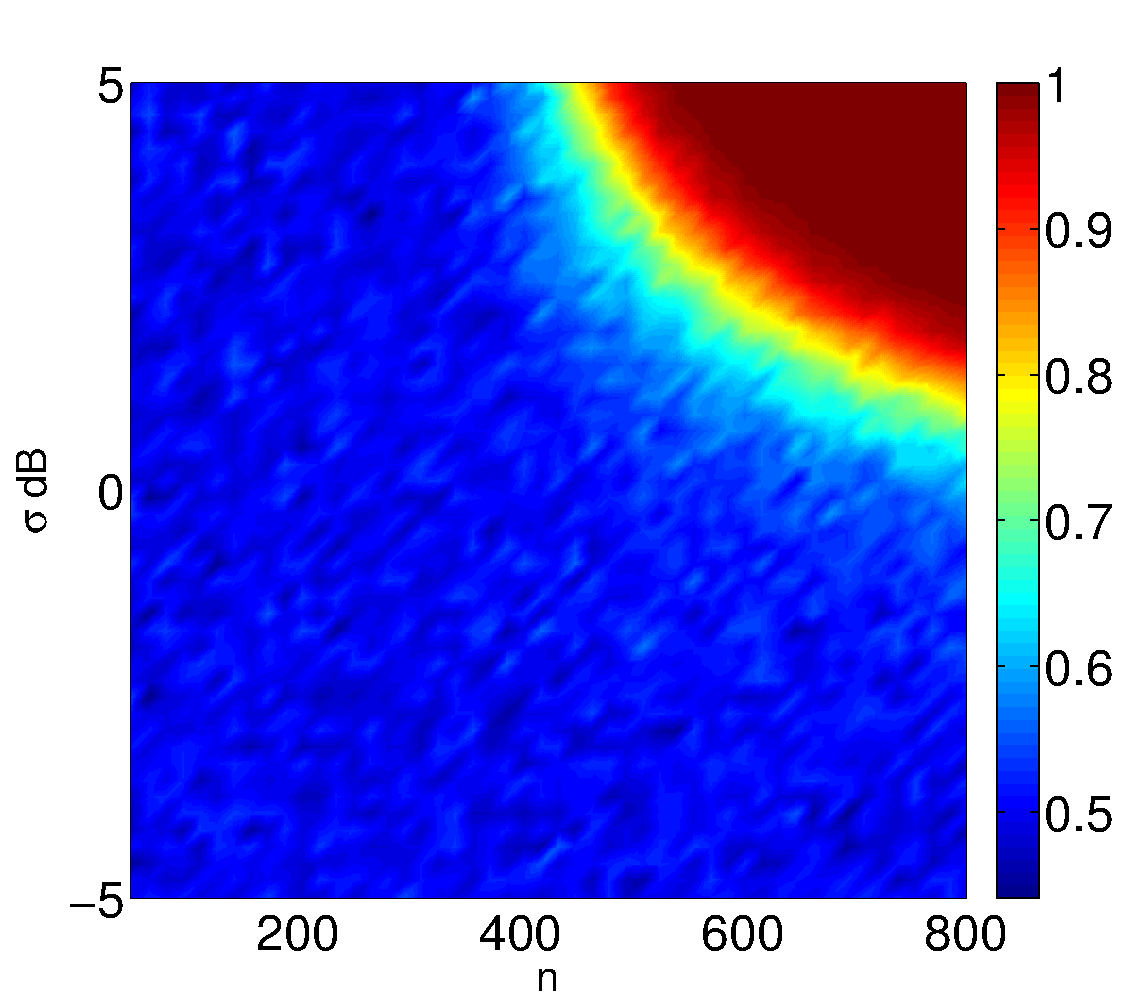
\includegraphics[width=\figwidth]{figures/cca_auc_heatmap.pdf}
  \caption{AUC for a detector based on the top singular value of $\widehat{C}$ in
    (\ref{eq:cca_chat_svd}) to detect the noise and signal data models in
    (\ref{eq:cca_data_model1}). Simulations were conducted using $d_1=200$, $d_2=150$, 500
    trials, and $\rho=0.9$.}
  \label{fig:cca_auc_heatmap}
\end{figure}

This is a new result. While the AUC heatmap in Figure \ref{fig:cca_auc_heatmap} closely
resembles the KS statistic heatmap in Figure \ref{fig:cca_ks_heatmap}, it also provides
information on how far the distributions are separated. When the distributions are
entirely separated, perfect detection is possible, resulting in an AUC of 1. This occurs
for large values of $n$ and $\sigma$. The AUC plot also confirms that when $n<d_1+d_2$,
CCA cannot statistically detect signals given correlated datasets. In fact, a large
portion of the parameter sweep of $n$ and $\sigma$ results in CCA failing.

The breakdown point when $n<d_1+d_2$ is an extremely undesirable property of CCA. In the
low-sample, high dimensional regime, it results in CCA being unable to detect the presence
of a signal given correlated datasets. We demonstrated through numerical simulation that
in this regime the distribution of the leading singular value of noise only datasets is
identical to that of datasets generated with correlated signal. However, using results
from random matrix theory, it is possible to avoid this undesirable performance loss.

\section{Informative CCA (ICCA)}

In \cite{nadakuditi2011fundamental}, Nadakuditi uses recent results from random matrix
theory to derive an informative version of CCA that we will call here informative CCA
(ICCA). Recalling the data SVDs $Y_1=U_1\Sigma_1V_1^H$ and $Y_2=U_2\Sigma_2V_2^H$, random
matrix theory provides the important insight that not all of the right singular vectors
are informative. In particular the following proposition is repeated from
\cite{nadakuditi2011fundamental} for here for reference. Let $z_1=
\left[z_1^{(1)},\dots,z_1^{(n)}\right]^H$ be the correlated signal vector in the first
dataset. 
\begin{prop}\label{prop:raj}
  As $d_1$, $n\to\infty$ with $d_1/n\to c_1$,
  \be
  \left| \left\langle \frac{z_1}{\|z_1\|_2}, V_1(:,1)\right\rangle\right|\convas\begin{cases}
    \varphi_1 & \text{if } \sigma > c_1^{1/4}\\
    0 & \text{otherwise}\\
  \end{cases}, 
  \ee 
  where $\varphi_1:=\sqrt{1 -
    \left(c_1+\sigma^2\right)/\left(\sigma^2\left(\sigma^2+1\right)\right)}$
  \cite{nadakuditi2011fundamental}.
\end{prop}
The analogous theorem holds for the second dataset. The notation $V_1(:,1)$ denotes the
first column of $V_1$. This proposition tells us that there is a critical SNR
$\sigma_{\text{crit}}=\left(\frac{d_1}{n}\right)^{1/4}$ such that if
$\sigma>\sigma_{\text{cirt}}$ the first column of $V_1$ is informative and contains a
portion of the correlated signal $z_1$. However, if $\sigma<\sigma_{\text{crit}}$ the
first column of $V_1$ is uninformative and contains no correlated signal. Such
uninformative components should not be used in CCA as they will degrade its
performance. Following \cite{nadakuditi2011fundamental}, we define the trimmed data
matrices as 
\be\ba
& \widetilde{U}_1 = U(:,1:r_1) && \widetilde{V}_1 = V(:,1:r_1)\\
& \widetilde{U}_2 = U(:,1:r_2) && \widetilde{V}_2 = V(:,1:r_2)\\
\ea\ee 
where $r_1$ and $r_2$ are the number of informative components in the first
and second datasets, respectively.Using these trimmed data matrices, we form the matrix
used for ICCA,
\beq\label{eq:icca_chat}
  \widetilde{C} = \widetilde{U}_1\widetilde{V}_1^H\widetilde{V}_2\widetilde{U}_2^H.
\eeq
Let $\widetilde{C} = \widetilde{F}\widetilde{K}\widetilde{G}^H$ be the SVD of this
matrix. ICCA returns the following informative correlation estimate and canonical vectors
\begin{equation}\label{eq:icca_rho}
\ba
&\widetilde{\rho} &&= \widetilde{k}_1\\
&\widetilde{x}_1 &&= \RIhat^{-1/2}\widetilde{f}_1\\
&\widetilde{x}_2 &&= \RIIhat^{-1/2}\widetilde{g}_1\\
\ea
\end{equation}
We next demonstrate that the correlation estimate returned by ICCA is superior to that
returned by CCA. 

\subsection{Simulation results}

We use the same simulation setup as in the CCA analysis, generating $n$ samples for each
dataset under both the noise and signal model in (\ref{eq:cca_data_model1}). Instead, of
using the estimate $\widehat{C}$, we form the estimates $\widetilde{C}^{\text{noise}}$ and
$\widetilde{C}^{\text{signal}}$ as in (\ref{eq:icca_chat}). First we explore the
distributions of the top singular value, $\widetilde{\rho}^{\text{noise}}$ and
$\widetilde{\rho}^{\text{signal}}$ of these matrices in Figure \ref{fig:icca_errorbars}.

\begin{figure}[h!]
  \centering
  \subfigure[$\sigma=0$ dB]{
    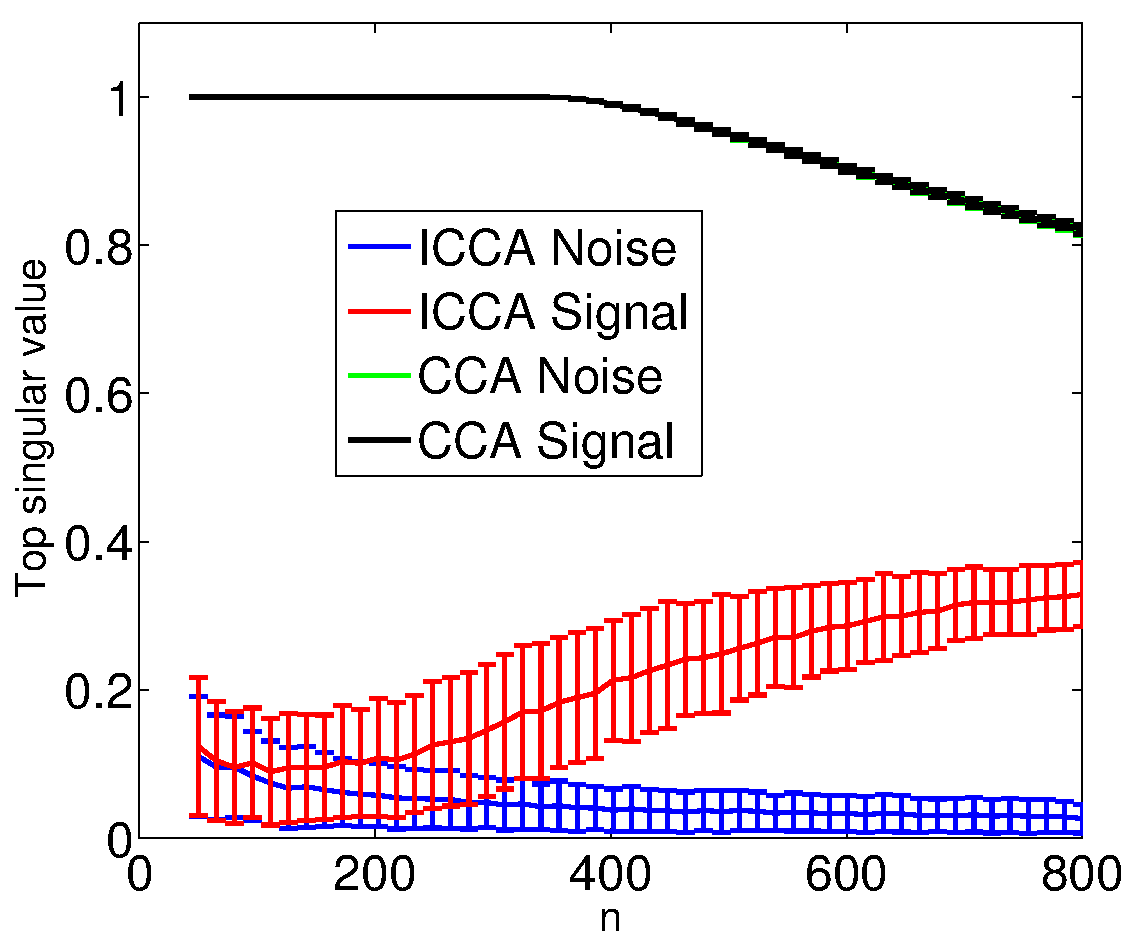
\includegraphics[width=\figwidth]{figures/icca_errorbars_low.pdf}
    \label{fig:icca_errorbars_low_snr}
  }
  \subfigure[$\sigma=3$ dB]{
    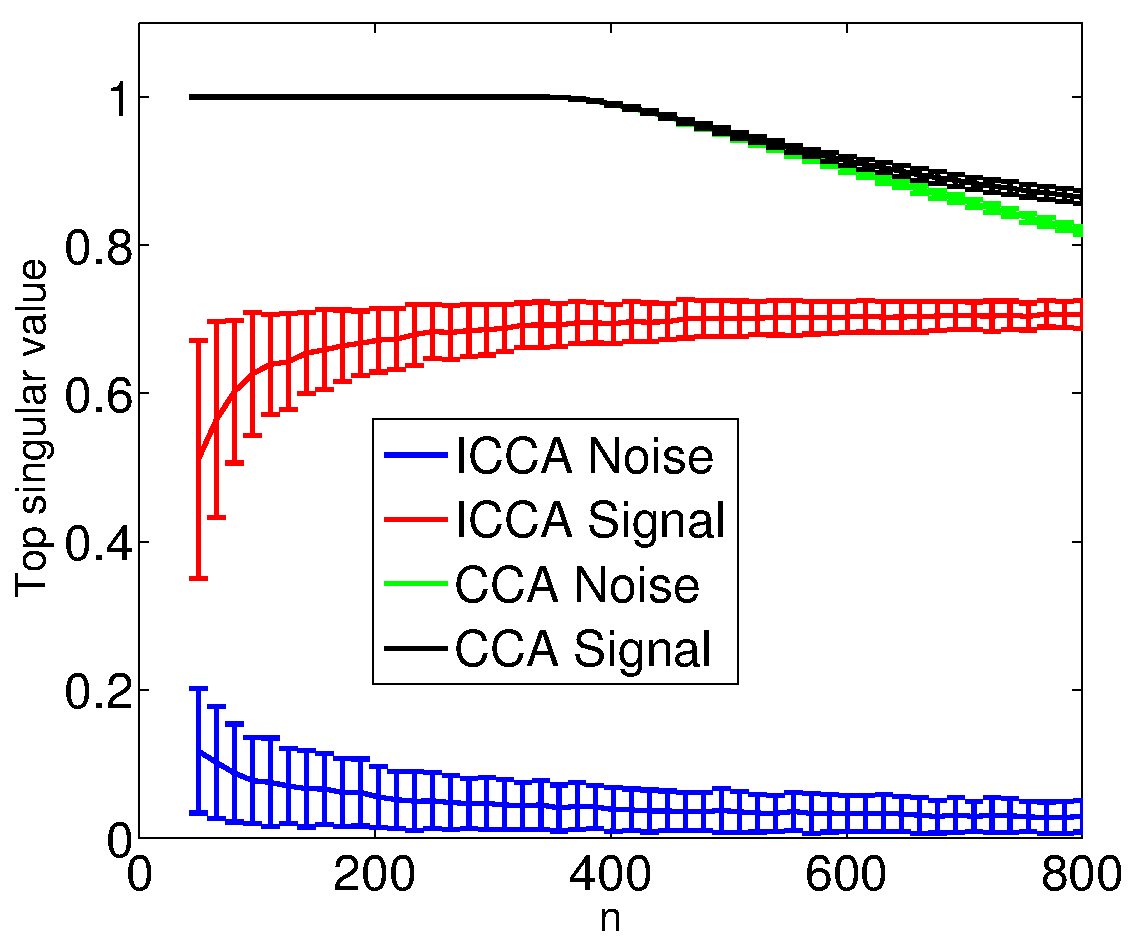
\includegraphics[width=\figwidth]{figures/icca_errorbars_high.pdf}
    \label{fig:icca_errorbars_high_snf}
  }
  \caption{Empirical distribution of the top singular value of $\widetilde{C}$ in
    (\ref{eq:icca_chat}) for both noise and signal data models in
    (\ref{eq:cca_data_model1}). Simulations were conducted using $d_1=200$, $d_2=150$,
    $\rho=0.9$, and $r_1=r_2=1$. The top singular value was computed for 500 trials. The
    mean top singular value is plotted with $\pm$ one standard deviation errorbars.}
  \label{fig:icca_errorbars}
\end{figure}

The results of the empirical distribution of the top singular value of $\widetilde{C}$ are
new. We immediately see many desirable characteristics of ICCA. First, the value of the
top singular value is no longer deterministically 1 when $n<d_1+d_2$. Second, as the
number of available training samples increases, $\tilde{\rho}^{\text{signal}}$ increases
for both values of $\sigma$.  This is desirable because it indicates that with more data,
the estimator is more confident that there is correlation between the dataset. Similarly,
with less data, the estimator is less confident that the datasets are correlated. As the
number of training samples increases, $\widetilde{\rho}^{\text{noise}}$ decreases to 0.
As the noisy datasets are uncorrelated ($\rho=0$), we would like the estimator to indicate
exactly this. The ICCA correlation estimate has this desirable property. Lastly, we note
that ICCA separates the distributions further and with less training data than CCA, even
under low SNR settings. Next, we use the KS statistic to explore when the empirical
distributions of $\widetilde{\rho}^{\text{noise}}$ and $\widetilde{\rho}^{\text{signal}}$
are statistically different. Results are shown in Figure \ref{fig:icca_ks_heatmap} with
the CCA KS heatmap presented again for ease of comparison.

\begin{figure}
  \subfigure[CCA]{
    \centering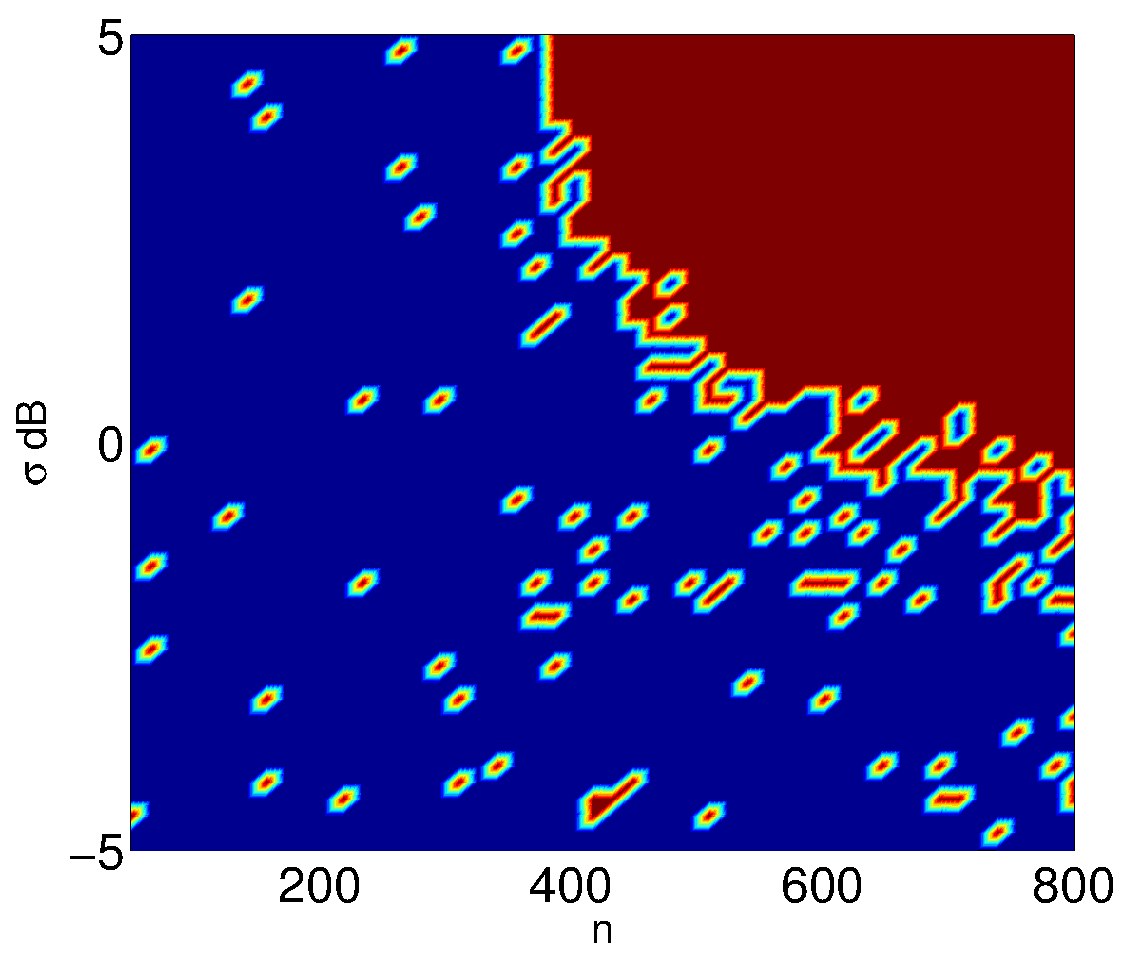
\includegraphics[width=\figwidth]{figures/cca_ks_heatmap.pdf}
  }
  \subfigure[ICCA]{
    \centering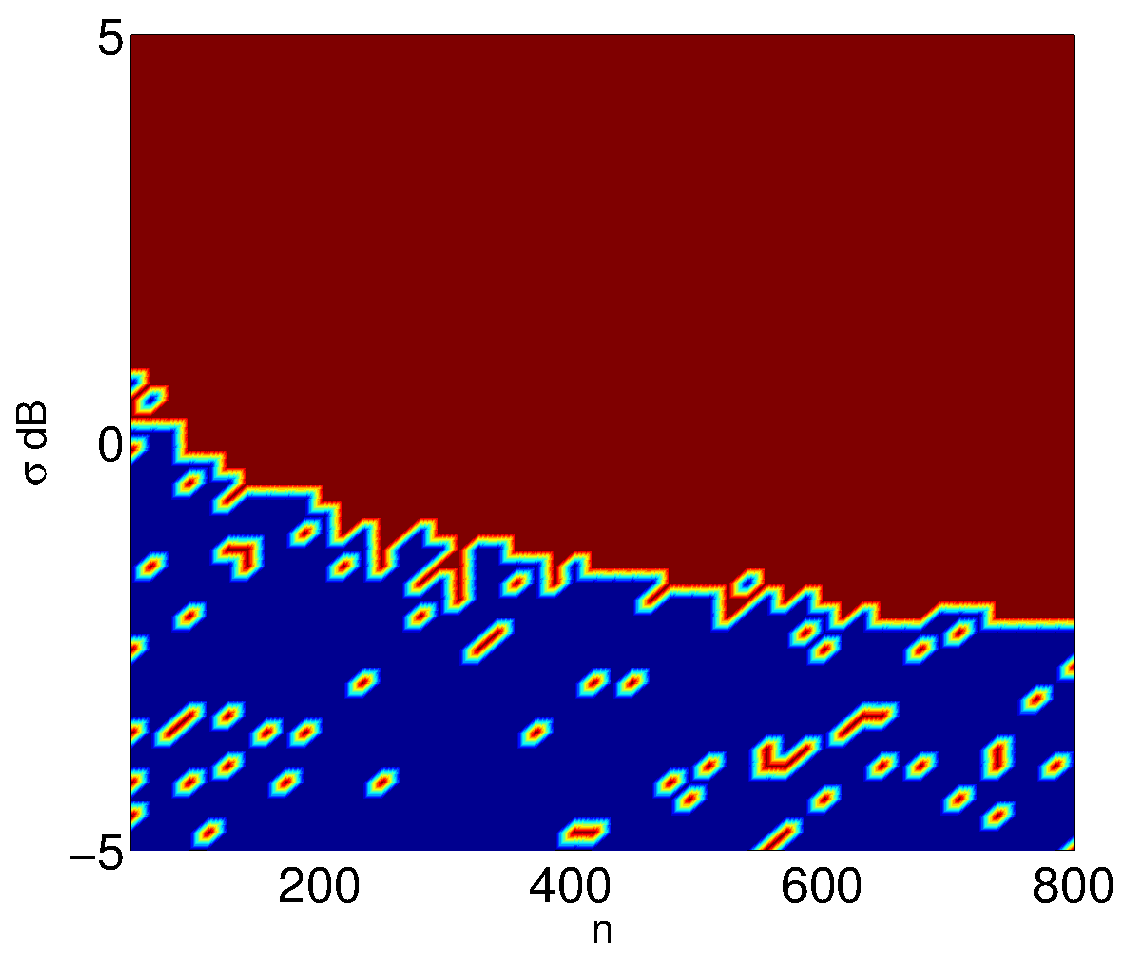
\includegraphics[width=\figwidth]{figures/icca_ks_heatmap.pdf}
  }
  \caption{Two-sided KS statistic between the empirical distributions of the leading
    singular value of $\widetilde{C}$ in (\ref{eq:icca_chat}) formed from training data
    generated from the noise and signal data models in
    (\ref{eq:cca_data_model1}). Simulations were conducted using $d_1=200$, $d_2=150$,
    $\rho=0.9$, $r_1=r_2=1$, 500 trials, and a significance level of $\alpha=0.95$ for the
    KS test. A value of 1 indicates the distributions are statistically different while a
    value of 0 indicates the distributions are statistically identical.}
  \label{fig:icca_ks_heatmap}
\end{figure}

This result confirms the result in \cite{nadakuditi2011fundamental}. Figure
\ref{fig:icca_ks_heatmap} shows that the empirical distributions of
$\widetilde{\rho}^{\text{noise}}$ and $\widetilde{\rho}^{\text{signal}}$ are statistically
different for a much larger number of combinations of $\sigma$ and $n$. In particular,
ICCA does not suffer from the performance breakdown at $n=d_1+d_2$ as CCA does. As one
would desire, given any number of training samples, the ICCA correlation estimates,
$\widetilde{\rho}^{\text{noise}}$ and $\widetilde{\rho}^{\text{signal}}$, are
statistically separable at a sufficiently large enough SNR. Intuitively, this SNR
threshold is larger for smaller values of $n$. For large $n$, ICCA can statistically
separate the distributions of $\widetilde{\rho}^{\text{noise}}$ and
$\widetilde{\rho}^{\text{signal}}$ at a lower SNR as compared to CCA. Finally, we explore
how separable these distributions are by examining the AUC for a na\"{\i}ve detector based
on the empirical correlation estimate returned by ICCA. These results are shown in Figure
\ref{fig:icca_auc_heatmap}. We present the AUC results from CCA again for ease of
comparison.

\begin{figure}
  \subfigure[CCA]{
    \centering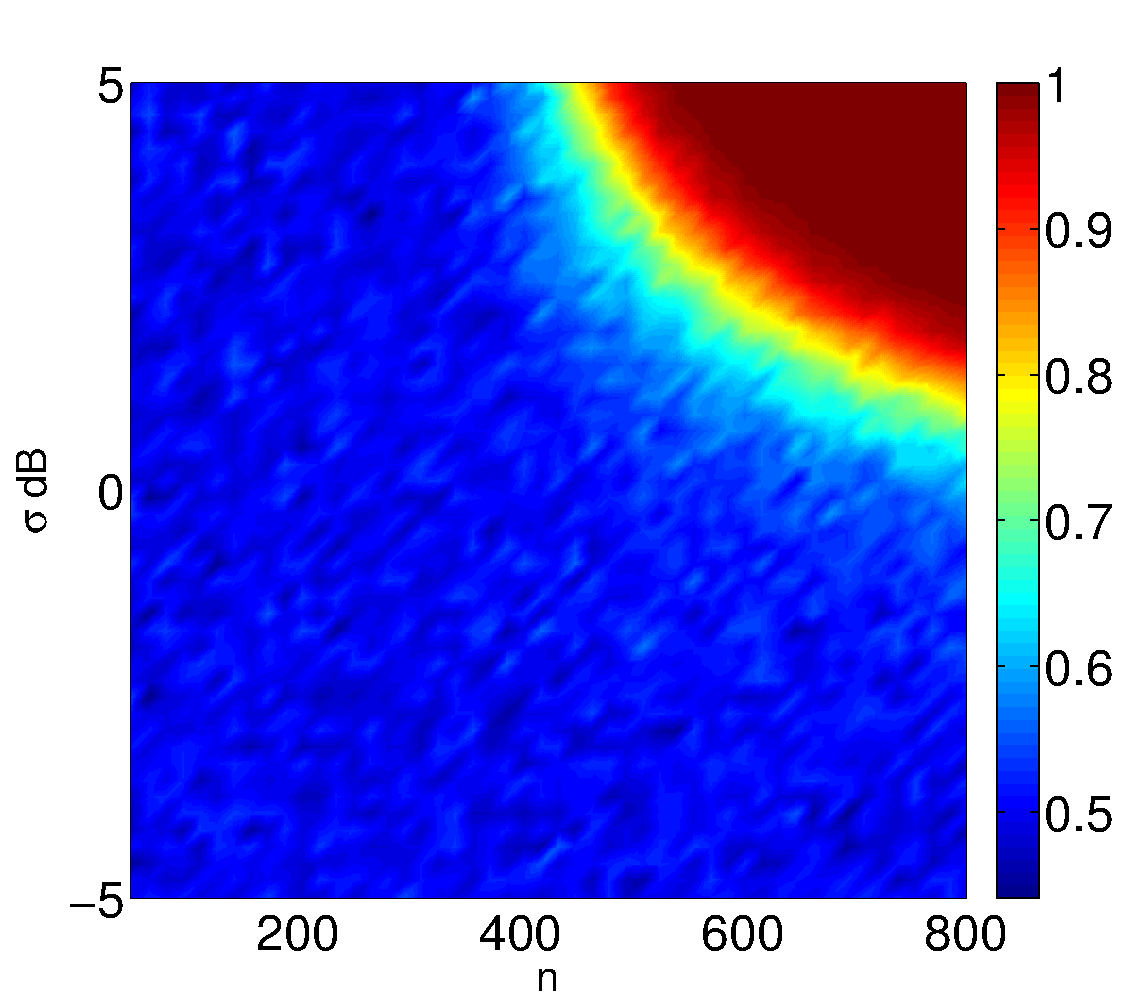
\includegraphics[width=\figwidth]{figures/cca_auc_heatmap.pdf}
  }
  \subfigure[ICCA]{
    \centering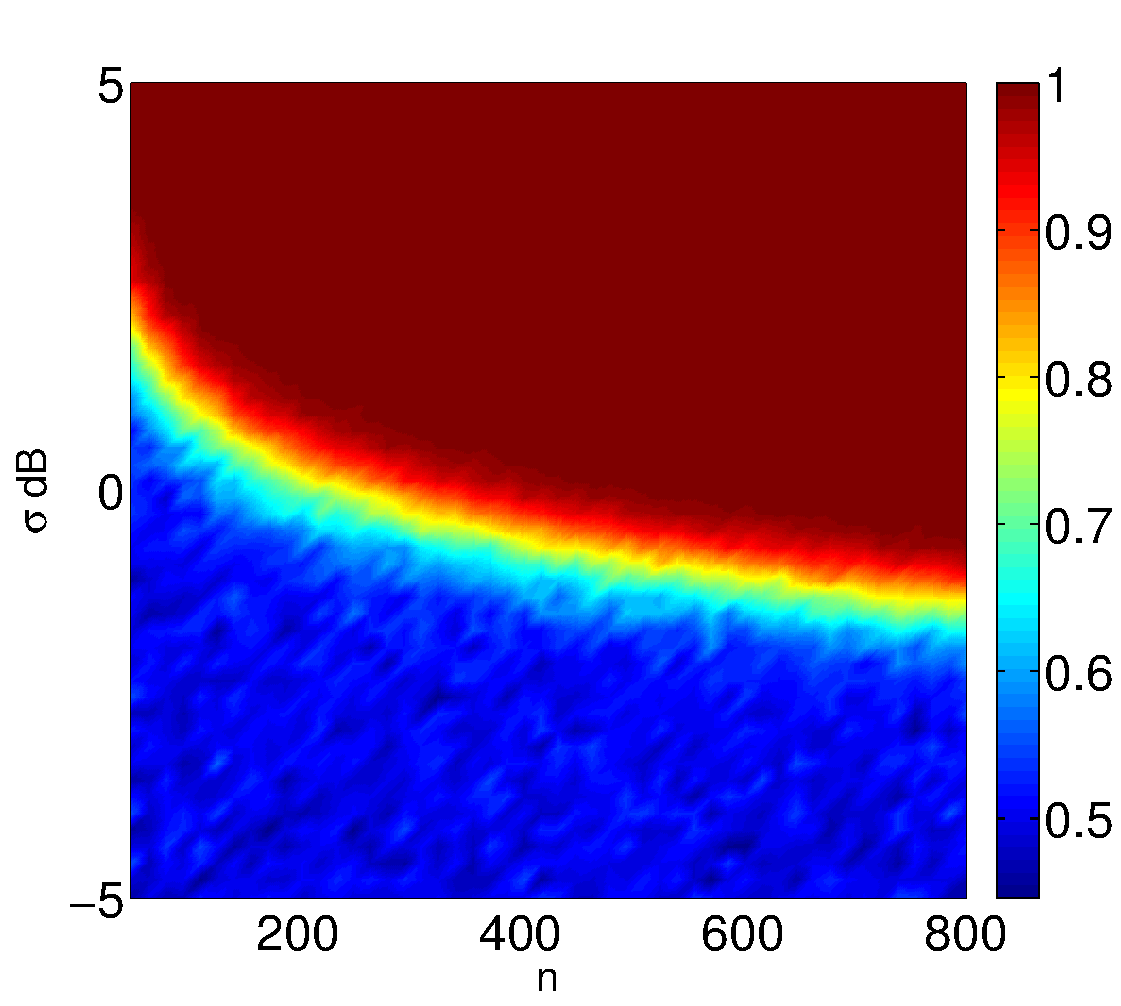
\includegraphics[width=\figwidth]{figures/icca_auc_heatmap.pdf}
  }
  \caption{AUC for a detector based on the top singular value of $\widetilde{C}$ in
    (\ref{eq:icca_chat}) to detect the noise and signal data models in
    (\ref{eq:cca_data_model1}). Simulations were conducted using $d_1=200$, $d_2=150$,
    $\rho=0.9$, 500 trials, and $r_1=r_2=1$.}
  \label{fig:icca_auc_heatmap}
\end{figure}

This is a new result. Similar to the KS statistic results in Figure
\ref{fig:icca_ks_heatmap}, the AUC results in Figure \ref{fig:icca_auc_heatmap} show that
ICCA outperforms CCA for a large number of combinations of $\sigma$ and $n$, most
importantly the sample starved regime. Again, for a fixed $n$, we observe a critical value
of $\sigma$, predicted by Proposition \ref{prop:raj}, above which signal detection is
possible. In the sample rich regime, ICCA can achieve perfect detection (AUC=1) for much
smaller values of SNR, which is highly desirable.

Clearly, the idea of trimming the training data SVDs to only include informative
components used in ICCA is beneficial. ICCA avoids the performance breakdown at
$n<d_1+d_2$ that is present in CCA. Furthermore, ICCA better separates the noise only and
signal distributions of the estimated correlation coefficient. Even in the sample rich
regime when many training data samples are available, ICCA is able to reliably detect
signals at a much lower SNR than CCA. CCA is not used often in the sample starved regime
because of this fundamental performance breakdown. Instead, it is common to use
regularized CCA (RCCA) in such a regime. In Chapter \ref{sec:rcca}, we explore the
performance of RCCA and apply the insights of informative data components to create an
informative version of RCCA. In the next chapter, we investigate applying CCA and ICCA to
matched subspace detection.
